\documentclass[12pt, letterpaper, titlepage]{article}

\usepackage{amsmath}
\usepackage{booktabs}
\usepackage{amsthm}
\usepackage{graphicx}
\usepackage[margin=1in]{geometry}
\usepackage{hyperref}
\hypersetup{colorlinks = true, linkcolor = blue, citecolor=blue, urlcolor = blue}
\usepackage{natbib}
\usepackage{enumitem}
\usepackage{setspace}

\usepackage[pagewise]{lineno}
%\linenumbers*[1]
% %% patches to make lineno work better with amsmath
\newcommand*\patchAmsMathEnvironmentForLineno[1]{%
 \expandafter\let\csname old#1\expandafter\endcsname\csname #1\endcsname
 \expandafter\let\csname oldend#1\expandafter\endcsname\csname end#1\endcsname
 \renewenvironment{#1}%
 {\linenomath\csname old#1\endcsname}%
 {\csname oldend#1\endcsname\endlinenomath}}%
\newcommand*\patchBothAmsMathEnvironmentsForLineno[1]{%
 \patchAmsMathEnvironmentForLineno{#1}%
 \patchAmsMathEnvironmentForLineno{#1*}}%

\AtBeginDocument{%
 \patchBothAmsMathEnvironmentsForLineno{equation}%
 \patchBothAmsMathEnvironmentsForLineno{align}%
 \patchBothAmsMathEnvironmentsForLineno{flalign}%
 \patchBothAmsMathEnvironmentsForLineno{alignat}%
 \patchBothAmsMathEnvironmentsForLineno{gather}%
 \patchBothAmsMathEnvironmentsForLineno{multline}%
}

% control floats
\renewcommand\floatpagefraction{.9}
\renewcommand\topfraction{.9}
\renewcommand\bottomfraction{.9}
\renewcommand\textfraction{.1}
\setcounter{totalnumber}{50}
\setcounter{topnumber}{50}
\setcounter{bottomnumber}{50}

\newcommand{\jy}[1]{\textcolor{blue}{JY: #1}}
\newcommand{\eds}[1]{\textcolor{red}{EDS: (#1)}}


\title{Sample Length at Which Block Bootstrapping is Effective for Estimation of Parameter of Time Series}

\author{Mathew Chandy\\
%   \href{mailto:mathew.chandy@uconn.edu}
% {\nolinkurl{mathew.chandy@uconn.edu}}\\
  Jun Yan\\[1ex]
  Department of Statistics, University of Connecticut\\
}
\date{}

\begin{document} 
\maketitle

\doublespace

\begin{abstract}
Block bootstrapping is a method that can be used for estimating a parameter of a time
series. It involves splitting a series into blocks (in order to account for the temporal dependence
factor) and re-sampling the blocks to create many new bootstrapped pseudo-samples of the time series.
This method becomes more effective as the length of the time series increases. 
The question that this study seeks to answer is what sample length is necessary for the block
bootstrap method to be effective in estimating a parameter of a time
series.

\bigskip
\noindent\sc{Keywords}:
block bootstrap;
\end{abstract}

\section{Introduction}
\label{sec:intro}

Block bootstrapping is a widely used method in Statistics. The concept for block 
bootstrapping was developed independently by \citet{hall1985resampling}, \citet{carlstein1986use}, and 
\citet{kunsch1989jackknife}. \citet{radovanov2014comparison} It has been applied to a variety of 
different domains such 
as econometrics \citep{mackinnon2006bootstrap} and meteorology \citep{varga2017generalised}. It can be used for 
situations in which there is temporal dependence within a population, and the goal is the estimation or testing a hypothesis about a parameter. Assuming that the sample is infinitely 
large, the method will work perfectly. However, for a finite sample size, the method will 
not work as well as expected. In the context of planning an applied 
statistical procedure, for which a large sample size is not always practical, it may be helpful to know how large the sample must be for the method to work at an acceptable level. 

\citet{hesterberg2015teachers} notes that while percentile-based confidence intervals from nonparametric bootstrapping are more accurate than t-intervals for larger sample sizes, they are less accurate for smaller sample sizes. \citet{nevitt2001performance} find that a sample size of 200-1000 is usually sufficient for estimation using the bootstrap method (simple resampling with no blocks involved). 
\citet{goncalves2005bootstrap} found that standard error estimates from block bootstrapping small 
samples may be significantly more accurate than inference from closed-form asymptotic estimates. That study focused on the estimation of a coefficient parameter within the context of linear regression. Still, the block bootstrap percentile confidence intervals under-covered the parameter even for n = 1024. 

The goal of this study is to find a threshold or range of sample sizes at which block bootstrap 
is an effective method for estimating a parameter in the context of a time series. The method is effective if approximately 1 - $\alpha$/2 \% of 1 - $\alpha$/2 \% of confidence intervals created from samples of the same size recover the parameter. This study will focus on estimating parameters of an AR(1) process with several types of confidence intervals from the literature, \citep{diciccio1996bootstrap}  \citep{rice2006mathematical} which will be reviewed in Section 2.

%At the base level, we are block-bootstrapping an auto-regressive process with true mean 0, and some AR(1) coefficient.

%Bootstrapping is the procedure of creating new pseudo-samples of the same size by resampling observations with replacement from the original sample. Basic bootstrapping works well for samples
% that are do not have a dependence factor. However, for a time series such as an auto-regressive or moving-average process, a different procedure is required to account for the time dependence. In such a situation, instead of resampling observations, blocks of the original sample can be resampled (these blocks must be of a certain length by which the sample length is divisible) to create a pseudo-sample. Point estimates of a parameter calculated from many block bootstrapped pseudo-samples are then used to create a distribution to create an interval estimation of the parameter.

%In this experiment, the mean, auto-correlation function (with a maximum lag of 1), and variance of a 1000 block-bootstrapped time series samples are computed, and 95\% confidence intervals of these parameters is created. 

%The various ways which these intervals can be constructed are described in \citet{diciccio1996bootstrap} and \citet{rice2006mathematical}. They will be discussed later in a review of the block bootstrap method. For the purposes of this study (in which the true parameters are known), in order to establish whether or not the method is effective, the block bootstrapping of a simulated sample can be replicated many times, and the proportion of confidence intervals that recover the true known parameter (coverage rate) is recorded. The goal of this is simply to observe how successful the block bootstrapping procedure is at estimating a parameter. The key variable being observed was, the sample length (n). It is known that as n increases, block bootstrapping should become a more accurate and precise method for estimation(the coverage rates will approach the theoretical confidence level and the interval widths will decrease). The question is what is the minimum sample length necessary to reach a coverage rate of 1 - $\alpha$/2 \%.

% In this experiment, there are certain variables that are expected to affect the performance of block bootstrap. As the the time dependence (AR or MA coefficient) of the time series increases, we expect the coverage rates of the confidence intervals to decrease.The coverage rates are also affected by the size of the blocks - more specifically,how the size of the blocks (l) relates to the size of the time series (n) - and whether or not they overlap. It is known that as the size of the time series increases, the optimal block length should increase, and the ratio of the block length to the time series length should decrease. l = n$^{1/3}$ is typically considered the optimal block length according to asymptotic theory. \citep{buhlmann1999block} Therefore, simulations in this study were conducted using this optimal function of l = n$^{1/3}$. 

%In order to solve the question of what sample length is necessary for effective block bootstrapping while still accounting for all these factors, the simulations were repeated for different variations of the MA coefficient, target parameter, and non-moving vs moving method. For each of these variations, results for block bootstrap estimation of mean, MA coefficient, and standard deviation were recorded for a wide range of sample length.

\section{Review of Block Bootstrap}
\label{sec:blkbootreview}

Block bootstrapping is a method that can be used to estimate a parameter of an AR(1) process. Suppose that one wants to estimate a parameter or parameters $\theta$ of an AR(1) process: 
\[X_{t} = \mu + \epsilon_{t} + \phi*X_{t-1}.\] The first step is to generate a sample of length $n$ from the process. An estimate of the parameter $\hat{\theta}_{n}$ can be computed from this sample. A pseudo-estimate $\hat\theta_n^*$ can be computed from a bootstrapped pseudo-sample. The mean $\bar\theta_n^*$ of many (typically 1000) replicate $\hat\theta_n^*$ can also be computed. Lastly, for each $\hat\theta_n^*$, $\delta = \hat\theta_n^* - \hat{\theta}_{n}$ and $\delta^* = \hat\theta_n^* - \bar\theta_n^*$ can be computed.

In regular bootstrap procedure, the new pseudo-sample of the same size as the original sample would be created by simply resampling observations from the original sample with replacement. In the case of a time series, in order to account for the temporal dependence, the time series can be split into blocks, typically of the same size. The block should be of size $l$ large enough to include time dependence, yet small enough to include some variance. As $n$ increases, an ideal $l$ should also increase, but the ratio of $l$ to $n$ should decrease. To achieve this, $l$ is often assigned a value as a function of $n$. A common function that is considered the best by much previous literature is $l = \lceil = n^{1/3} \rceil$. \citep{buhlmann1999block} A bootstrapped sample is created by taking a sample of $n / l$ blocks with replacement to create a new pseudo-sample of size $n$. The designer of the study can choose whether the blocks overlap or not. If the blocks can never overlap, it is called a non-moving block bootstrap. In this case, the original sample is split evenly into $n / l$ blocks, and the same number of blocks are sampled with replacement to create a bootstrapped pseudo-sample. If the blocks do overlap, it is called a moving block bootstrap. $n / l$ samples are taken randomly from the original sample, but they do not have to be from a set of evenly spaced blocks. $\hat\theta_n^*$ is computed from the pseudo-sample. This procedure can be repeated many times to create a distribution of $\hat\theta_n^*$. 

In this study, 1000 bootstrapped $\hat\theta_n^*$ were created for each simulation. Using this distribution of $\hat\theta_n^*$, a $1 - \alpha$/2 \% confidence interval for the parameter can be created. The most simplistic method for constructing this interval is the percentile confidence interval. For a parameter $\theta$, the percentile $1 - \alpha$/2 \% confidence interval takes the form: 
\[ [\hat\theta_{n, \alpha/2}^*, \hat\theta_{n, 1 - \alpha/2}^*].\] 
Another method is the bias-corrected and accelerated 
(BCA) $1 - \alpha$/2 \% confidence interval, which takes the form: 
\[ [\hat\theta_{n, \alpha_1}^*,\hat\theta_{n, \alpha_2}^*].\] 
$\alpha_{1}$ and $\alpha_{2}$ are the cumulative probability of $z_{1}$ and $z_{2}$, respectively, where:
\[z_{1} = \frac{z_{0} - z_{1 - \alpha/2}}{1 - a(z_{0} - z_{1 - \alpha/2})} + z_{0}\] and
\[z_{2} = \frac{z_{0} + z_{1 - \alpha/2}}{1 - a(z_{0} + z_{1 - \alpha/2})} + z_{0}.\] 
Where $z_0$ is the quantile function of the proportion of $\hat\theta_n^* < \bar\theta_n^*$, and $a$ is the skewness of ...
	
	Both of these intervals are good at recovering the mean and standard deviation of a temporally dependent process, but their coverage of the temporal dependence deteriorates as $n$ increases. A potential solution to this issue is to center the intervals around either $\hat{\theta}_{n}$ or $\bar\theta_n^*$. To do this, the distribution of $\delta$ or $\delta^*$ should be considered. A percentile interval centered around $\hat{\theta}_{n}$ takes the form:
\[ [\hat{\theta}_{n} + \delta^*_{\alpha/2}, \hat{\theta}_{n} + \delta^*_{1 - \alpha/2}].\] 
A percentile interval centered around $\bar\theta_n^*$ takes the form: 
\[ [\bar\theta_n^* + \delta_{\alpha/2}, \bar\theta_n^* + \delta_{1 - \alpha/2}].\]
An alternative is an interval of the form:
\[ [\hat{\theta}_{n} - \delta^*_{1 - \alpha/2}, \hat{\theta}_{n} - \delta^*_{\alpha/2}],\] 
which is equivalent to:
\[ [\hat{\theta}_{n} + \bar\theta_n^*- \hat\theta_{n, \alpha/2}^*, \hat{\theta}_{n} + \bar\theta_n^* - \hat\theta_{n, 1 - \alpha/2}^*],\] 
and therefore is also equivalent to:
\[ [\bar\theta_n^* - \delta_{1 - \alpha/2}, \bar\theta_n^*- \delta_{\alpha/2}].\] 
Thus, the interval is centered around both $\hat{\theta}_{n}$ and $\bar\theta_n^*$.

This centering procedure can also be applied to a BCA interval. A BCA interval centered around $\hat{\theta}_{n}$ takes the form:
\[ [\hat{\theta}_{n} + \delta^*_{\alpha_1}, \hat{\theta}_{n} + \delta^*_{\alpha_2}].\] 
A BCA interval centered around $\bar\theta_n^*$ takes the form: 
\[ [\bar\theta_n^* + \delta_{\alpha_1}, \bar\theta_n^* + \delta_{\alpha_2}].\]
An alternative is an interval of the form:
\[ [\hat{\theta}_{n} - \delta^*_{\alpha_2}, \hat{\theta}_{n} - \delta^*_{\alpha_1}],\] 

\section{Simulation Study}
\label{sec:simstudy}

%The central objective of the study was to assess what sample size is necessary for the the block bootstrap method to estimate a parameter of an autoregressive process. The method will work better as the sample size goes to infinity, but the goal is to see what is the smallest sample size that is acceptable. The sample size is acceptable if many 1 - $\alpha$/2 confidence intervals for that sample size recover the parameter at a rate of 1 - $\alpha$/2 \%. In the previous section, the procedures for creating three types of confidence interval of a parameter using the block bootstrap method are described. 

%These procedures are applied to a simulation of an autoregressive integrated moving average (ARIMA) process to create three confidence interval of certain parameters (the mean, the AR(1) coefficient, the MA(1) coefficient, the standard deviation, etc.). 

R has a built in function that allows you to simulate an AR(1) process, for which one can set the theoretical $\phi$. For the purposes of this study, $\mu$ should be fixed at 0, and the standard deviation of the process $\sigma_{x}$ should be fixed at 1. By default, the standard deviation of the error term $\sigma_{\epsilon}$ is 1, so the observations can be multiplied by $\sqrt{1 - \phi^2}$ so that the new theoretical $\sigma_{x}$ is equivalent to 1, as shown below:

\[X_{t} = \epsilon_{t} + \phi*X_{t-1}.\]
\[Var(X_{t}) = Var(\epsilon_{t} + \phi*X_{t-1})\]
\[\sigma^2_{x} = \sigma^2_{\epsilon} + \phi^2*\sigma^2_{x}\]
\[\sigma^2_{x}(1 - \phi^2) = \sigma^2_{\epsilon}\]
\[\sigma_{\epsilon} = \sigma_{x}\sqrt{1 - \phi^2}\]

The only parameter of the AR(1) process that was varied was $\phi$, as the temporal dependence affects the performance of block bootstrap. $\phi$ = 0 (a standard normal distribution), 0.2, and 0.4 were used in this study. 

As described in the last section, the block bootstrap method can be used to estimate a parameter $\theta$ of an AR(1) process. In this study, $\theta$ is composed of the target parameters $\mu$, $\sigma_{x}$, and $\phi$. From a sample of length $n$, six block bootstrap 95\% confidence intervals can be constructed for each target parameter: ....

Each of these 18 intervals either recovers $\theta$ or does not. Remember that 95\% of a certain type of 95\% confidence intervals constructed from samples of the same $n$ should recover $\theta$. To see if this is approximately the case, one can run 1000 replications of the block bootstrap procedure, and for each interval-$\theta$ pair, the rate at which that type of interval recovers $\theta$ can be recorded.


If $\theta$ is not covered at that $n$, a larger sample size must be necessary. $n = 100, 200, 300, 400, and 500$ were used in this study. 

%For all simulation studies, but $\mu$ and $\sigma_{x}$ can be kept constant, but increasing temporal dependence factors such as AR and MA Coefficients can make block bootstrap less effective in estimation, so its impact on the method's performance should be analyzed. For a certain variation of an AR(1) process, block bootstrap 95\% confidence intervals for each of 3 parameters ($\mu$, $\sigma_{x}$, and the autocorrelation function$\rho$) can be replicated for 1000 simulated samples of a certain length. For each individual confidence interval, it can be recorded whether or not the interval includes the true parameter. The coverage rate, or the proportion of intervals that include the true parameter, can then be recorded. If the parameter is being properly estimated by the block bootstrap, the coverage rate should reflect this by being close to the confidence level of 95\%. If this is not the case, the method is not working as well as it should. The width of the confidence interval for each replication is dependent on the variability of the parameter of the time series. If the interval is on average not wide enough to capture the parameter at the expected rate of 95\%, it indicates that the variability of the parameter is underestimated. If the interval is too wide and captures the parameter at a rate above 95\%, it indicates that the variability of the parameter is overestimated. Since the coverage rate is a proportion based on 1000 independent binary outcomes (the interval recovers the parameter or it doesn't), a 95\% confidence interval of the coverage rate for each parameter can also be created. The inclusion of .95 in the interval indicates that the block bootstrap method is working well for its respective parameter. If this is not the case for this sample length, the procedure can be conducted again with a larger sample length. This can be repeated until the method is determined to be working acceptably, meaning that .95 is included in the 95\% confidence interval of the coverage rate of the parameter.



%1000 replicates of length-n random samples of an AR(1) process with theoretical $\mu$ = 0, $\sigma_{x}$ = 1, and $\theta$ = 0.1 were simulated using R. For each of three target parameters ($\mu$ = 0, $\sigma_{x}$ = 1, and $\theta$ = 0.1, three types of block bootstrap (with block length l) confidence intervals (percentile, empirical, and BCA) were constructed for each replicate sample. The statistic used to estimate $\mu$ is the sample mean $\bar{x}$, the statistic used to estimate $\sigma$ is the sample standard deviation $S^2$, and the statistic used to estimate $\theta$ is the auto-correlation function of the sample. For each of these nine categories of confidence intervals, the coverage rate of its respective parameter was computed, along with a 95\% confidence interval of the proportion given 4000 trials. For a certain variation of the process, the study was repeated for n = 125, 1000, 3375, and 8000. The only parameter of the process that was varied was $\theta$, and 0.1, 0.3, and 0.5 were the values used.



\begin{figure}[tbp]
\caption{}
  \centering
  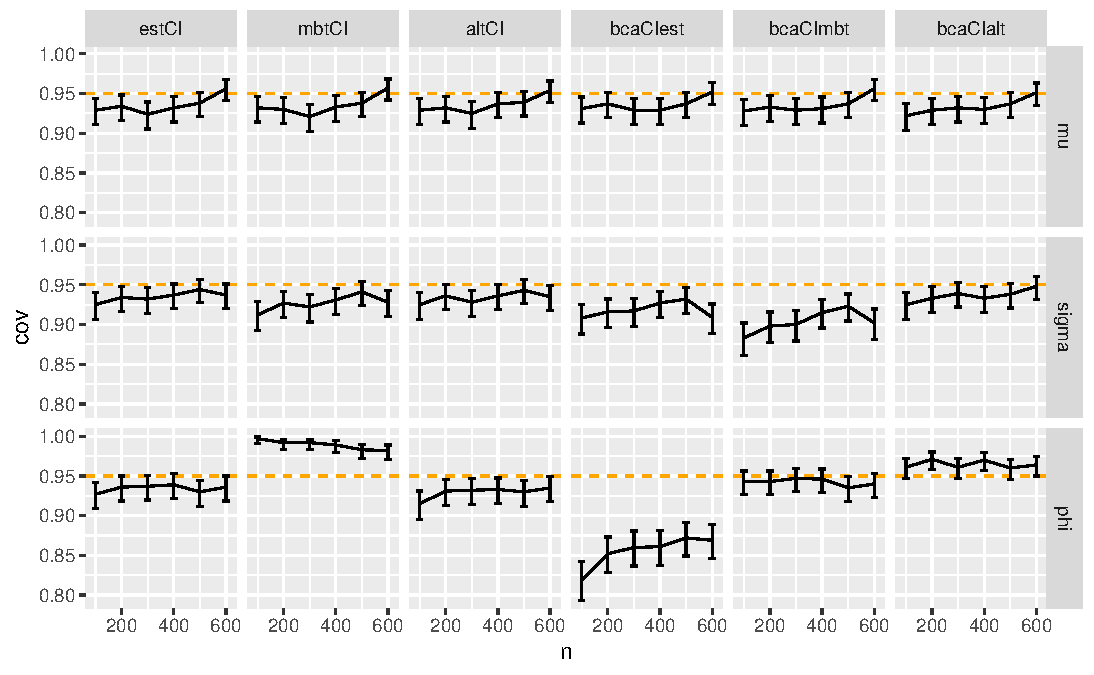
\includegraphics[width=\textwidth]{figures/plot_0}
  \caption{At $\phi = 0$, all intervals covered $\mu$ correctly at $n = 500$. All but three intervals seem to cover $\phi$ generally well for $n = 300$. The alternate percentile interval slightly under-covers $\phi$ for all sample lengths observed. The BCA interval centered around $\hat{\theta}_{n}$ significantly under-covers $\phi$ and the percentile interval centered around $\bar\theta_n^*$ over-covers $\phi$. All intervals seem to cover $\sigma$ generally well for n = 500 except for the $\hat{\theta}_{n}$-centered BCA interval, which slightly under-covers $\sigma$ for all sample lengths observed, and the  $\bar\theta_n^*$-centered BCA interval, which also under-covers $\sigma$.}
  \label{fig:plot_0}
\end{figure}

\begin{figure}[tbp]
\caption{}
  \centering
  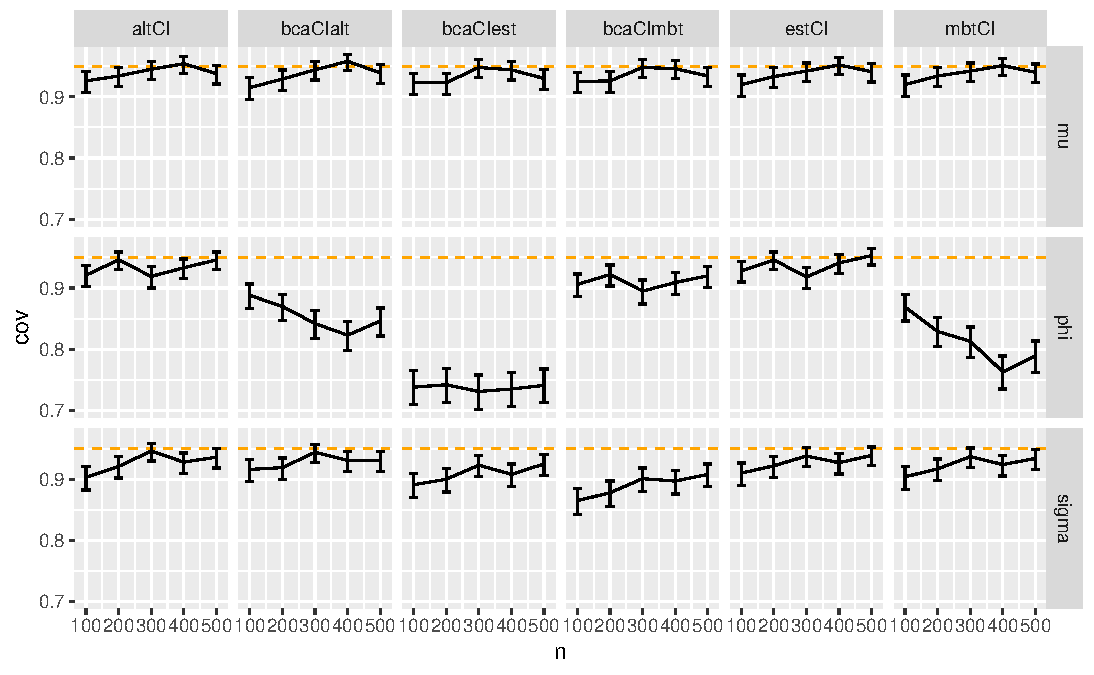
\includegraphics[width=\textwidth]{figures/plot_.2}
  \caption{At $\phi = .2$, all intervals covered $\mu$ correctly at $n = 300$ and $n = 400$. The alternate percentile interval and the $\hat{\theta}_{n}$-centered percentile interval cover $\phi$ well at $n = 500$. The $\bar\theta_n^*$-centered BCA interval slightly under-covers $\phi$ for all sample lengths observed. The alternate BCA interval under-covers $\phi$, and its performance deteriorates as $n$ increases, as does the $\bar\theta_n^*$-centered percentile interval but with lower coverage rates and more noticeable deterioration. The $\hat{\theta}_{n}$-centered BCA interval significantly under-covers $\phi$, although there is no clear deterioration.}
  \label{fig:plot_.2}
\end{figure}

\begin{figure}[tbp]
\caption{}
  \centering
  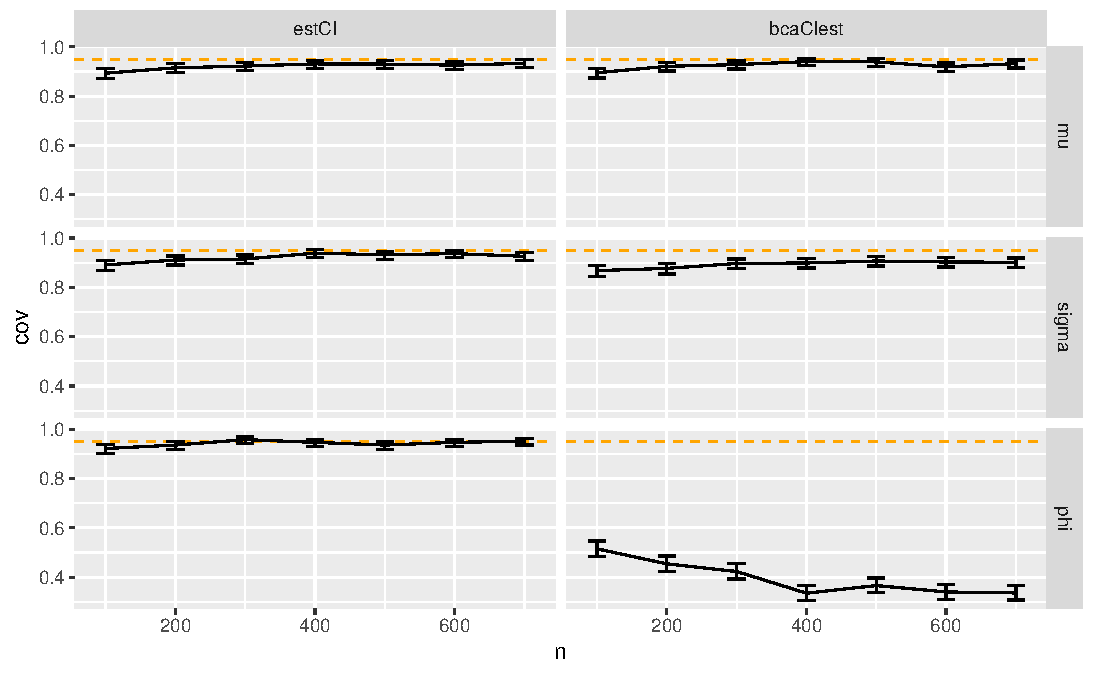
\includegraphics[width=\textwidth]{figures/plot_.4}
  \caption{At $\phi = .4$,}
  \label{fig:plot_.4}
\end{figure}

\section{Concluding Remarks}
\label{sec:conremarks}

This study finds that as the AR coefficient increases, the sample size necessary for effective block bootstrap estimation must be larger. When implementing the block bootstrap method to estimate the mean or variance of an autoregressive process, the non-moving method and moving method perform about the same. However, when estimating the AR(1) coefficient, the non-moving method performs noticeably worse than the moving method, which still covers the coefficient poorly when theta is greater than 0. Whereas the performance improves as sample length increases when the target is the mean or variance, the performance decays as sample length increases when the target is the AR(1) coefficient.


\bibliographystyle{chicago}
\bibliography{citations}[tp]


\end{document}